\section{\astarix Algorithm: Optimizations} \label{sec:optimizations}
We now discuss several optimizations we developed to speed up \astarix while
preserving its optimality. These optimizations reduce preprocessing and
alignment runtime as well as memory footprint (in particular for memoization).

\subsection{Reducing Semi-global to Local Alignment Using a Trie} \label{TRIEsubsec:trie}
To find an optimal alignment, we generally need to consider all reference graph
nodes $u \in \RG$ as possible starting nodes. Thus, optimal aligners
\pasgal~\cite{jain_accelerating_2019} and
\bitparallel~\cite{rautiainen_bitparallel_2019} brute-force through all
possible starting nodes $u \in \RG$.

To more efficiently handle arbitrary starting positions for alignments, we
extend the reference graph with a trie (referred to as \textit{suffix tree}
in~\cite{dox2018efficient}) to effectively align from all possible starting
nodes \emph{simultaneously}.

\para{Single Starting State}
In the trie approach, abstraction nodes are added to the graph, each of which
corresponds to a set of nodes in $\RG$ that correspond to the same prefix. In
the following, we formalize this approach.

Concretely, we extend $\RG$ by a \emph{trie of depth $D$}, resulting in graph
$\TG=(\TGV,\TGE)$. Our goal is that all paths in $\RG$ that have length $D$ and
end in $v \in \RGV$ correspond to paths in $\TG$ starting from a single source
$\epsilon$ to $v \in \TGV$, where $\epsilon$ represents the empty string. This
correspondence ensures that it suffices to consider only paths in $\TG$ starting
from the source $\epsilon$. In particular, each alignment on $\TG$ can
be translated into an alignment on $\RG$ (we omit this translation
here).

\begin{wrapfigure}{r}{0.48\linewidth}
	%\vspace{-20pt}
	\centering
	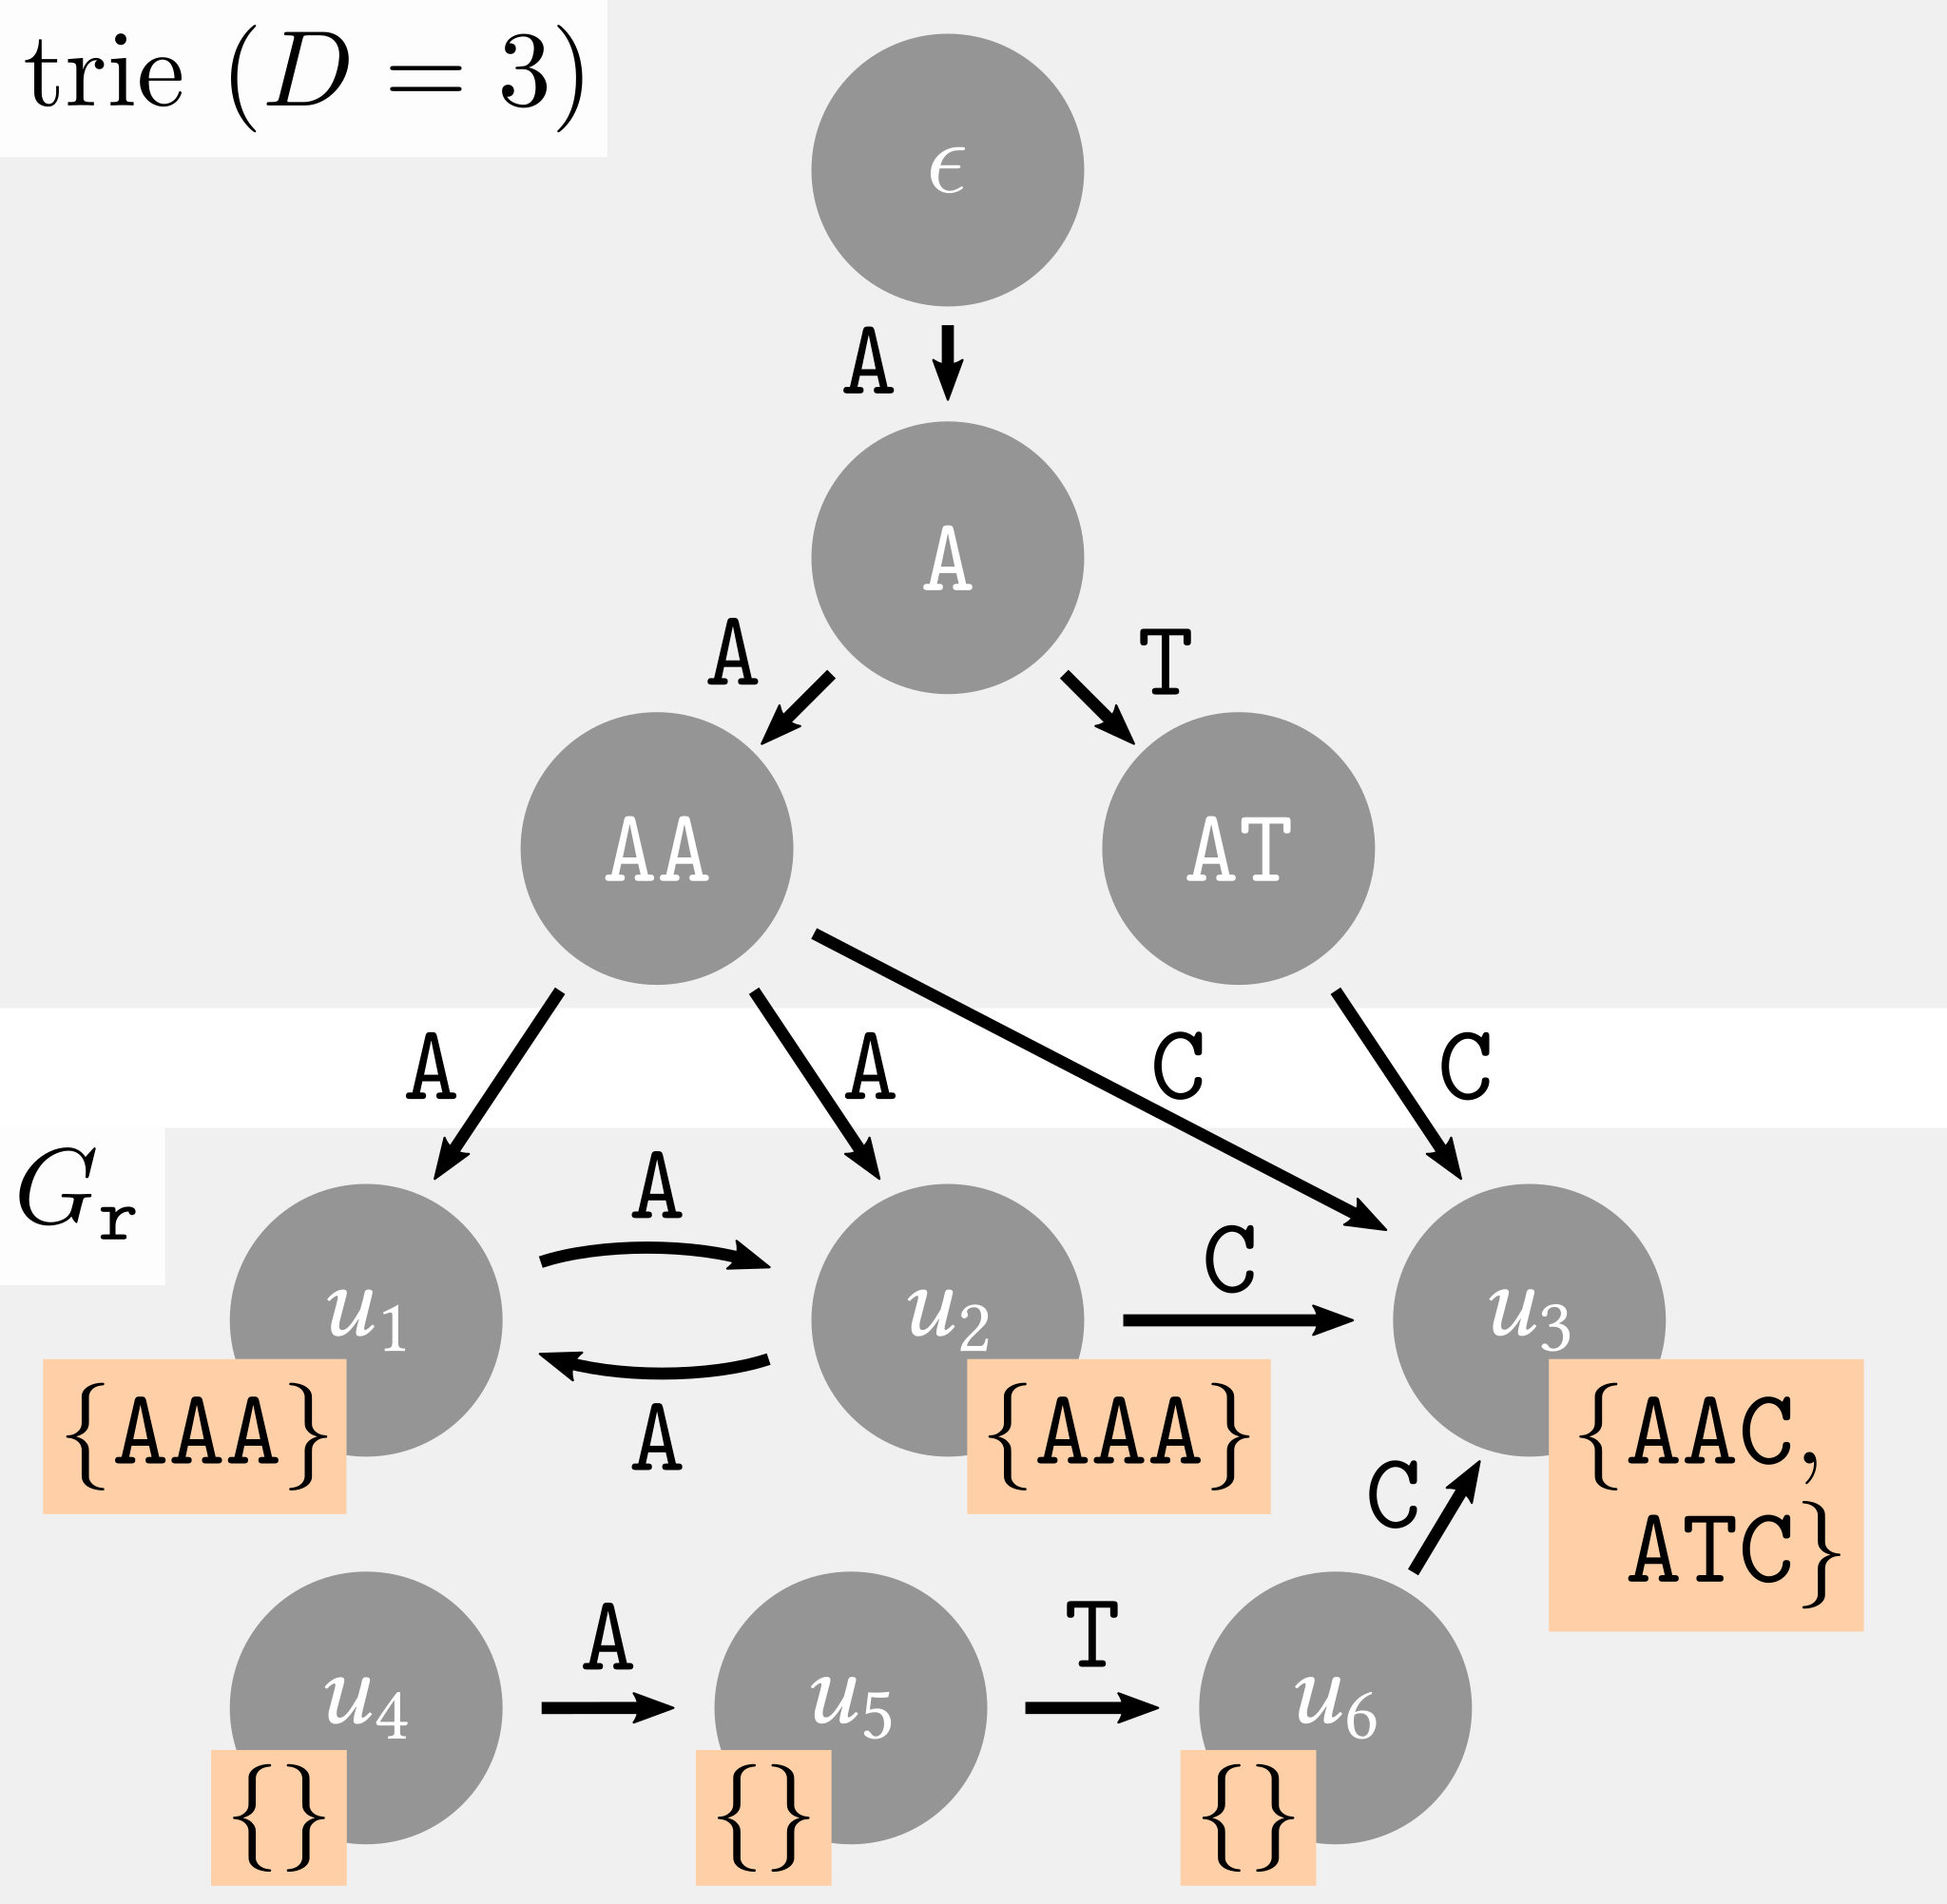
\includegraphics[width=\linewidth]{figs/tree}
	\caption{$\TG$ enables semi-global alignment by extending $\RG$ with a trie.}
	\label{TRIEfig:trie}
	\vspace{-25pt}
\end{wrapfigure}
\cref{TRIEfig:trie} shows an example trie. To construct it, we first associate with
every node $v \in \RGV$ the set $\mathcal{S}_v$ of its $D$-mers (orange boxes in
\cref{TRIEfig:trie}): spells of paths ending in $v$ and of length $D$. Our goal is
then to use paths in the trie to spell these $D$-mers.

Second, we construct the trie nodes from all prefixes of these $D$-mers:
%
$$ \TGV:= \RGV \cup
\bigcup_{v \in \RGV} \left\{s[0:i] \,\middle|\, \begin{array}{c}
	s \in \mathcal{S}_v, \\
	0 \leq i < D
\end{array} \right\}.
$$

Third, we add edges within the trie, which ensure that paths from $\epsilon$ to
any trie node $s$ spell $s$. Formally, whenever $s \concat \ell \in \TGV$, we add
an edge $(s,s \concat \ell, \ell)$ to $\TGE$, where ``$\concat$'' denotes string
concatenation.
%
Finally, we add edges between the trie and the reference graph, which ensure
that any $D$-mer of any node $v \in \RGV$ can be spelled by a walk from
$\epsilon$ to $v$. Formally, if $s \concat \ell \in \mathcal{S}_v$, then
$(s,v,\ell) \in \TGE$.

Importantly, extending $\RG$ to $\TG$ is compatible with the construction of the
edit graph $\EG$, the construction of the alignment graph and all other
optimizations. In particular, when searching for a shortest path in the
alignment graph constructed from $\TG$, it suffices to only consider starting
node $\langle \epsilon, 0 \rangle$.

\para{Reducing Size of Trie} \label{TRIEpara:reducing_trie}
We can reduce the size of the trie by removing specific trie nodes.
%
In particular, we iteratively remove each trie leaf node $s \cdot \ell \in \TGV$ with a unique outgoing edge $(s \cdot \ell, v, \ell')$ to a reference graph node $v \in \RGV$.
%
To compensate for removing node $s \cdot \ell$, we introduce a new edge $(s, u, \ell)$ to a node $u \in \RGV$ with an edge $(u,v,\ell')$ (such a node must exist according to the construction of $\TG$).
%
For example, in \cref{TRIEfig:trie}, we (i)~remove node \texttt{AT} including its edges $(\texttt{A},\texttt{AT},\texttt{T})$ and $(\texttt{AT},u_3,\texttt{C})$, but (ii)~introduce an edge $(\texttt{A},u_2,T)$.

This optimization is lossless, as the $D$-mer $s \cdot \ell \cdot \ell' \in \mathcal{S}_v$ can still be spelled by the path from $\epsilon$ to $s$, extended by $(s, u, \ell)$ and $(u, v, \ell')$.

\subsection{Greedy Match Optimization} \label{subsec:greedy}
We also employ an optimization originally developed for computing the edit
distance between two strings~\cite{sellers_algorithm_1974,allison_lazy_1992}, but
which has also been used in the context of string to graph
alignment~\cite{dox2018efficient}. We omit the correctness proof of this
optimization, which is already covered
in~\cite{sellers_algorithm_1974}, and only explain the intuition behind it.

Suppose there is only one outgoing edge $e = (u, v, \ell) \in \RGE$ from a node
$u \in \RGV$. Suppose also that while aligning a query $q$, we explore state
$\st{u}{i}$ for which the next query letter $q[i]$ matches the label $\ell$. In
this case, we do not need to consider the edit outgoing edges, because
any edit at this point can be postponed without additional cost, as $\cmatch
\leq \min(\csubst, \cins, \cdel)$. Thus, we can greedily explore state
$\st{v}{i+1}$, aligning $q[i+1]$ to $e$ by using the edge $(\st{u}{i},
\st{v}{i+1}, \ell, \cmatch)$ before continuing with the \A search.
We note that this optimization is only applicable when aligning in non-branching
regions of the reference graph. In particular, it is not applicable for most
trie nodes (\cref{subsec:trie}).

\subsection{Speeding Up Evaluation of Heuristic} \label{subsec:speedup-heuristic}
In the following, we show how to reduce the runtime of evaluating the heuristic
$h(u,s)$, by introducing two separate optimizations that compose naturally.

\para{Capping Cost} We cap $h(u,s)$ at $\costcap$, replacing it by
$h_{\costcap}(u,s):=\min(h(u,s),\costcap)$. To achieve this, we allow
\textsc{RecursiveAlign} to ignore paths costing more than $\costcap$.
%
For large enough $\costcap$, this speeds up computation without significantly
decreasing the benefit of the heuristic, since nodes associated with a high
heuristic value are typically not explored anyways. We investigate the effect of
$\costcap$ in \cref{subsec:parameter_estimation}.

\begin{samepage}
	\begin{theorem} \label{thm:hbar_optimistic}
		$h_{\costcap}$ is optimistic.
	\end{theorem}
	\begin{proof}
		We have $h_\costcap(u,s) \leq h(u,s)$ and that $h(u,s)$ is
		optimistic (\cref{thm:optimistic}).
	\end{proof}
	\end{samepage}

\para{Capping Depth}
We reduce the number of nodes that need to be considered by $h(u,s)$. To this
end, we define a modified heuristic $h_d(u,s)$ that only considers nodes $R_u
\subseteq \EGV$ at distance at most $d$ from $u$ (cp. \cref{lin:d} in
\cref{alg:astarix}):
$
R_u := \{ v \in \RGV \mid \exists \; \text{path } \pi \in \EG \text{ from } u \text{ to } v \text{ with } \lvert \pi \rvert \leq d \}
$.

If an alignment of $s$ reaches the boundary of $R_u$, defined as $$B(R_u) := \{v
\in R_u \mid \exists (v,v',\ell) \in \EGE \text{ with } v' \notin R_u \},$$ it is
allowed to only spell a prefix of $s$, and the remaining unaligned letters of
$s$ are considered aligned with zero cost:
\begin{gather*}
h_d(u,s) := \min_{\pi \in \Pi} \cost{\pi}, \text{ where } \\
\Pi := \left\{ \pi \in \RG \;\middle|\; \begin{array}{c}
\mli{start}(\pi)=u, 
\sigma(\pi)=s \lor \big(\mli{end}(\pi)\in B(R_u) \land \exists i. \sigma(\pi)=s[1..i] \big)
\end{array}
\right\}
\end{gather*}

\begin{samepage}
\begin{theorem} \label{thm:hbar_optimistic}
	$h_d$ is optimistic.
\end{theorem}
\begin{proof}
It suffices to show $h_d(u,s) \leq h(u, s)$ since $h(u, s)$ is optimistic. In
the case where all of $s$ is aligned, $h_d(u,s) = h(u, s)$. Otherwise, the
unaligned letters of $s$ are not penalized, so $h_d(u,s) \leq h(u, s)$.
\end{proof}
\end{samepage}


\subsection{Partitioning Nodes into Equivalence Classes} \label{subsec:partition}
We have shown in \cref{para:memoization} how to reuse an already computed
$h(u,s)$ for repeating $s$ across different queries and query positions. In the
following, we additionally aim to reuse $h(u,s)$ across different nodes $u$, so
that $h(u,s)$ does not need to be computed for all nodes $u$. Intuitively, we
want to assign two nodes $u$ and $v$ to the same equivalence class when the
\emph{graph region} considered by $h(u,s)$ is equivalent to the graph region
considered by $h(v,s)$, up to renaming of nodes.

Thus, $h(u,s)=h(v,s)$ if $u$ and $v$ are from the same equivalence class.
Therefore, we can (arbitrarily) choose a representative node $r \in \RGV$ for
every equivalence class, and evaluate $h(r,s)$ instead of $h(u,s)$, where $r$ is
the representative of the equivalence class of $u$. To look up representative
nodes in $\Oh(1)$, we define a helper array $\mli{repr}$ with $\mli{repr[u]} =
r$.

\para{Identifying Equivalence Classes}
To identify the nodes belonging to the same equivalence class, we assume the
optimization from \cref{subsec:speedup-heuristic}, i.e., that our heuristic only
considers nodes up to a distance $d$ from~$u$.
%
Moreover, for performance reasons, our implementation detects only the
equivalence classes of nodes $u$ with a single outgoing path of length at least
$d$.
%
In this case, $u$ and $u'$ are in the same equivalence class if their outgoing
paths spell the same sequence.
%
In contrast, we leave nodes with forking paths in separate equivalence classes.

Note that for smaller $d$, the number of equivalence classes gets smaller, the
reuse of the heuristic gets higher, and the memoization table has a lower memory
footprint. At the same time, however, the heuristic $h_d(u,s)$ is less
informative.
